\documentclass{article}
\usepackage{amsmath}
\usepackage{graphicx}

\title{Notes on the Distribution Function}
\author{Prof. Marco Panesi \\
\emph{Center for Hypersonics and Entry Systems Studies (CHESS)}\\
\emph{University of Illinois}}
\date{}

\begin{document}


\maketitle



\tableofcontents

\vspace{0.5cm}

In kinetic theory, the distribution function is a crucial concept that is used to describe how the velocities of particles in a dilute gas are distributed at any given time. These notes introduce the fundamentals of the distribution function and its applications in the context of particle motion and collisions. Key topics covered include the mathematical formulation of the distribution function, differential fluxes of molecules, momentum, and energy, and the treatment of molecular collisions, such as elastic collisions and their role in determining equilibrium states like the Maxwell-Boltzmann distribution. Furthermore, models like the hard-sphere and \emph{Variable-Hard-Sphere} (VHS) models are discussed, providing insights into how collision rates and cross sections are computed in gas dynamics. For more in-depth details, please refer to the provided references.


\section{Distribution Function: The Basics}
In this so-called \emph{velocity space} the molecule is thus represented by a point located at the end of the velocity vector $C_i$ laid off from the origin. The entire gas in the volume V is represented correspondingly by a cloud of N points in this space.\\

The number of particles number of particles of class $C_i$ in the volume element dV$_C$ is
$$
dn = n f(C_i) dV_C
$$
The distribution function \( f(C_i) \) gives the fraction of molecules in class \( C_i \), that is, the fraction with velocity in the range \( (C_i, C_i + dC_i) \). This function is fundamental in kinetic theory to describe how molecules are distributed in terms of their velocities.

\[
f(C_i) dV_c = \text{fraction of molecules in class } C_i \text{ with velocities in the range } (C_i, C_i + dC_i)
\]

Here, \( C_i \) is a vector representing the components of the velocity in three Cartesian coordinates:

\[
C_i \equiv (C_1, C_2, C_3)
\]

The volume element \( dV_c \) in velocity space can be written in two coordinate systems:

\begin{itemize}
    \item In \textbf{Cartesian coordinates}, it is given by:
    \[
    dV_c = dC_1 \, dC_2 \, dC_3
    \]
    \item In \textbf{Spherical polar coordinates}, the volume element is:
    \[
    dV_c = C^2 \, dC \, \sin(\theta) \, d\theta \, d\phi
    \]
    where \( C \) is the magnitude of the velocity, \( \theta \) is the polar angle, and \( \phi \) is the azimuthal angle.
\end{itemize}

\begin{figure}
        \centering
        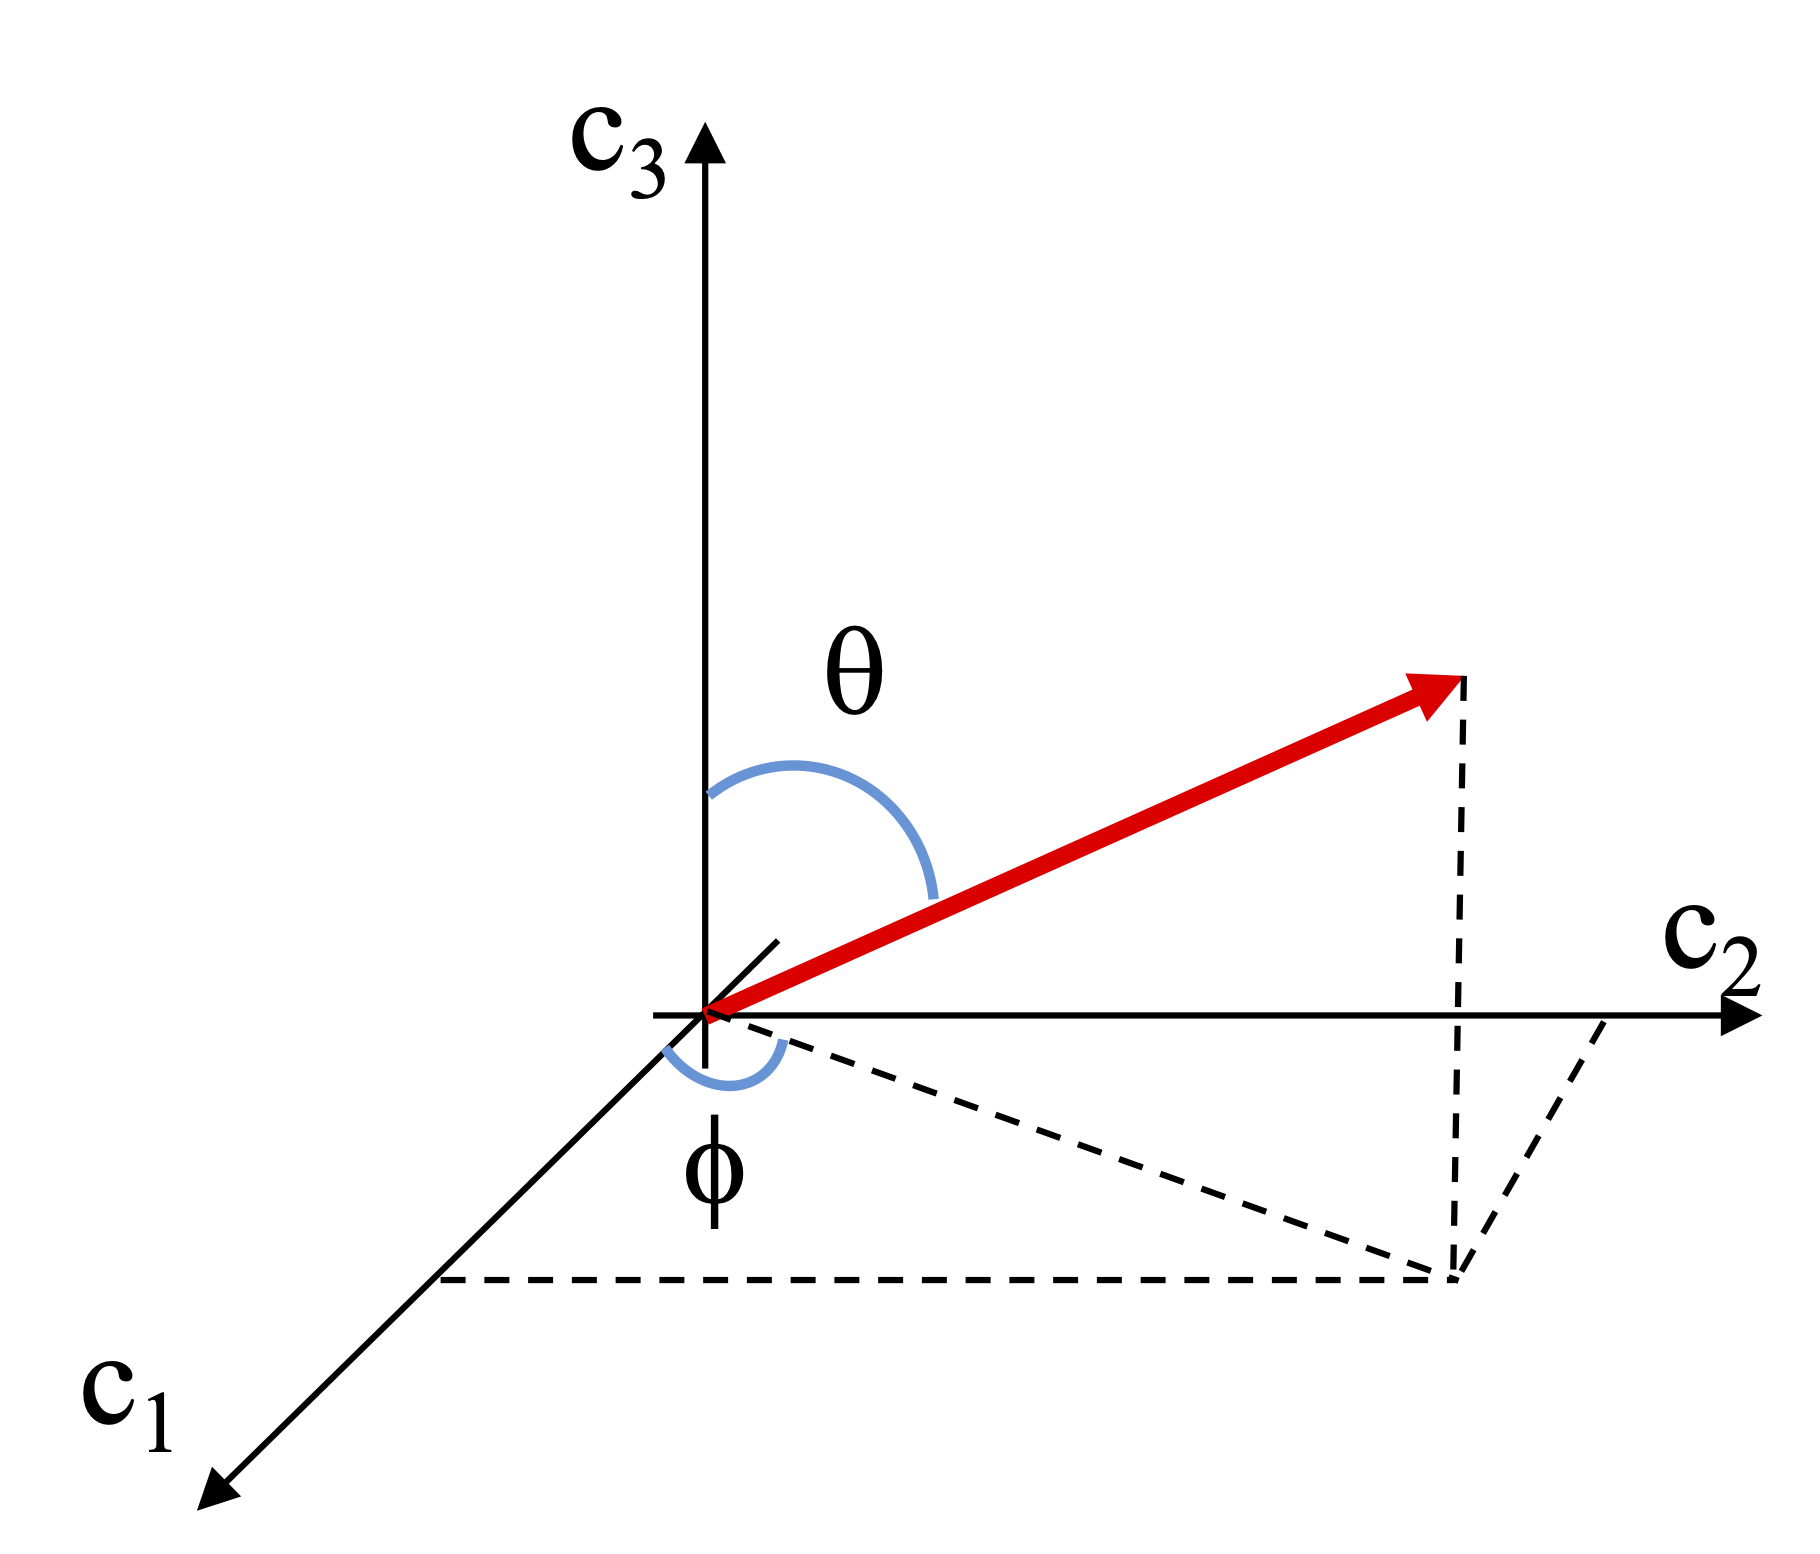
\includegraphics[width=0.45\textwidth]{coord.png}
        \caption{Cartesian and Spherical Coordinates}
    \end{figure}
    
\paragraph{Differential number flux}  The flux of molecules is denoted by \( \phi_k^{(n)} \), which is defined as the number of molecules crossing a unit area per unit time in the direction \( x_k \). Mathematically:

\[
\phi_k^{(n)} = \frac{\# \text{ of molecules}}{\text{time} \times \text{area in direction } x_k}
\]

The differential flux of molecules traveling in the direction \( k \) is:

\[
d^{(3)}\phi_k^{(n)} = n \, (C_i \cdot \hat{i}_k) \, f(C_i) \, dV_c
\]

where:
\begin{itemize}
    \item \( n \) is the number density,
    \item \( \hat{i}_k \) is a unit vector in the \( k \)-direction,
    \item \( f(C_i) \) is the distribution function of molecules with velocity \( C_i \),
    \item \( dV_c \) is the differential volume element in velocity space.
\end{itemize}

For example, the differential flux in the \( x_2 \)-direction is:

\[
d^{(3)}\phi_2^{(n)} = n \, C_2 \, f(C_i) \, dV_c
\]

Here, \( C_2 \) is the \( x_2 \)-component of the velocity vector \( C_i \), and \( d^{(3)}\phi_2^{(n)} \) represents the differential flux of molecules in class \( C_i \) traveling in the \( x_2 \)-direction.

\paragraph{Differential Fluxes of Momentum and Energy} One can construct differential fluxes of momentum and energy. The number flux and the energy flux are both vectors, where the direction of the vector represents the direction in which the transport occurs. Momentum transport occurs in a similar way and can be represented using similar expressions.

Number flux and energy flux are scalar vectors, where the direction of the vector indicates the direction of transport. Momentum flux, on the other hand, is a tensor. One "direction" is the momentum component, and the other is the direction in which this vector quantity is being transported.

\begin{itemize}
    \item \emph{Example 1}:
    \[
    d^{(3)}\phi_2^{(\epsilon)} = \frac{1}{2} m C^2 \, n C_2 \, f(C_i) \, dV_c
    \]
    This represents the differential kinetic energy flux in the \( x_2 \)-direction being transported by molecules of class \( C_i \). Here, \( \frac{1}{2} m C^2 \) is the kinetic energy of the molecules of class \( C_i \), and \( C_2 \) is the \( x_2 \)-component of velocity \( C_i \).
    
    \item \emph{Example 2}:
    \[
    d^{(3)}\phi_{12}^{(p)} = m C_1 \, n C_2 \, f(C_i) \, dV_c
    \]
    This represents the differential \( x_1 \)-momentum flux in the \( x_2 \)-direction, transported by molecules of class \( C_i \).
\end{itemize}

\section{Molecular Collisions}

\subsection{Collision Process}

A general collision between two molecules can be represented as follows:

\[
(C_i, Z_i) \longrightarrow (C'_i, Z'_i)
\]

Here, \( C_i \) and \( Z_i \) represent the initial states (\emph{i.e.}, velocities) of the two molecules before the collision, and \( C'_i \), \( Z'_i \) represent their final states after the collision. The equilibrium distribution is the velocity (or energy) distribution of particles that does not change over time, despite collisions occurring continuously. This occurs when the system has reached a state in which collisions do not further alter the statistical distribution of velocities or energies in the system. For instance, in a gas at equilibrium, the velocity distribution is given by the Maxwell-Boltzmann distribution.

\subsection{Definition of Cross Section}

Consider a uniform beam of test particles (labeled A) incident on a field particle (labeled 2), as illustrated schematically. Let \( n_B \) denote the number density of test particles in the beam, and \( g \) the relative velocity between the test particles and the field particle. The flux of test particles, \( \Gamma_1 \), is defined as the number of test particles crossing a unit area normal to the beam per unit time:

\[
\Gamma_B = n_B g.
\]

The total collision cross section \( \sigma_{AB}(g) \) between a test particle (A) and a field particle (B) is defined by the ratio of the number of collisions per unit time between the test particles and the field particle to the test particle flux:

\[
\sigma_{AB}(g) = \frac{\text{Number of collisions with field particle per unit time}}{\Gamma_B}.
\]

The dimensions of \( \sigma_{AB}(g) \) are:

\[
[\sigma_{AB}] = \frac{[\text{time}^{-1}]}{[\Gamma_{AB}]} = [L^2],
\]

indicating that the total cross section has units of area. Physically, the cross section represents the effective geometrical "blocking area" that the field particle presents to the beam of test particles. This quantity is a function of the relative speed \( g \) and depends on the types of particles involved in the collision. For hard-sphere interactions, the cross section is independent of the order of the subscripts, meaning \( \sigma_{AB}(g) = \sigma_{AB}(g) \).\\

The cross section is often interpreted geometrically as the area around a field particle within which a test particle must pass to result in a collision, and it is commonly used to compute collision rates and related properties in kinetic theory.

\begin{figure}
        \centering
        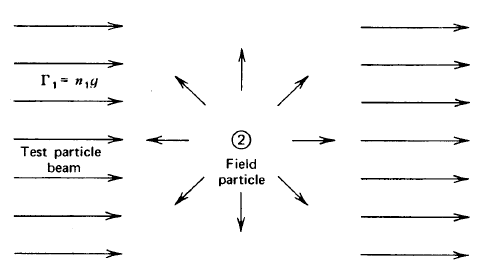
\includegraphics[width=0.6\textwidth]{crossSec.png}
        \caption{Cartesian and Spherical Coordinates}
    \end{figure}

\subsection{Definition of Collision Rate}

The collision rate quantifies how frequently collisions occur between two types of molecules, \( A \) and \( B \), within a given volume and time. The rate is given by:

\[
Z_{\text{AB}} = \frac{\text{Number of collisions}}{\text{Time} \times \text{Volume}}
\]

This is an important quantity for calculating macroscopic properties like reaction rates and transport coefficients (\emph{e.g.}, viscosity or thermal conductivity) in gases.

\subsection{Hard Sphere (HS) Model}

To model molecular collisions, a straightforward approach is to treat molecules as \emph{hard spheres}, similar to billiard balls. In this model, the molecules of type \( A \) and \( B \) have fixed radii, and a collision occurs when their centers come within a certain distance of each other. In a real (quantum) world of nuclei surrounded by swarms of electrons, things are not so clear-cut, and one must define probabilities of particular outcomes given specific inputs.

Let’s define the parameters:
\begin{itemize}
    \item \( m_A \), \( m_B \): masses of molecules A and B.
    \item \( d_A \), \( d_B \): diameters of molecules A and B.
    \item \( g_i = Z_i - C_i \): the relative velocity of molecule B with respect to molecule A before the collision.
\end{itemize}

We can imagine a sphere of radius \( d_{AB} \) surrounding the center of molecule A. If the trajectory of molecule B brings its center inside this sphere, a collision will occur between A and B. The cross-sectional area of this sphere is the target area for the collision, and if the relative velocity \( g_i \) is directed inside this area, a collision will occur.
A collision occurs when the distance between the centers of the molecules is less than the sum of their radii, \( d_{AB} \), given by:

\[
d_{AB} = \frac{d_A + d_B}{2}
\]

The \emph{collision cross-section}, denoted \( \sigma_t \), represents the effective area for a collision to occur. For hard spheres, the total collision cross-section is:

\[
\sigma_t = \pi d_{AB}^2
\]

This is a simplified model that is useful for understanding basic concepts in kinetic theory.\\

%\section*{Improved Collision Models}

While the hard-sphere model gives valuable insights, it often fails to accurately predict specific details, especially when dealing with real gases or plasmas where interactions are more complex. 

\subsection{Variable Hard Sphere (VHS) Model}

An improvement on the hard-sphere model is the \emph{Variable Hard Sphere (VHS)} model, which accounts for the fact that the collision cross-section depends on the relative velocity of the molecules. In the VHS model, the cross-section is a function of the relative speed \( g \):

\[
\sigma_t = \sigma(g)
\]

This model is more accurate for aerodynamics and gas dynamics calculations, especially in non-equilibrium conditions, such as those encountered in hypersonic flows or plasmas. For more complex cases, such as chemical reactions or quantum mechanical effects, even more sophisticated models are required.

%\section*{Elastic Collisions}

\subsection{Elastic Collision Definition}

An \emph{elastic collision} is one in which the total kinetic energy of the system remains constant. There is no loss of kinetic energy to promote changes in energy (such as molecular vibrations or rotations), and momentum is conserved. 

In an elastic collision between two molecules:
\[
g' = g
\]
where \( g' \) is the relative speed after the collision, and \( g \) is the relative speed before the collision. However, the relative \emph{velocity vector} can change direction. The scattering angles govern this change in direction.

\subsection{Scattering Angles and Cross Sections}

Two angles characterize the change in the direction of the relative velocity vector:
\begin{itemize}
    \item \( \chi \): the polar angle.
    \item \( \epsilon \): the azimuthal angle.
\end{itemize}

These angles define the orientation of the velocity vector after the collision $g_i'$, relative to its direction before the collision $g_i$. The differential solid angle \( d\hat{\Omega} \), which describes the infinitesimal changes of the angles $\chi$ and $\epsilon$, is given by:

\[
d\hat{\Omega} = \sin \chi \, d\chi \, d\epsilon
\]

The \emph{differential scattering cross-section} \( \frac{d\sigma}{d\Omega} \) represents the probability that a collision will result in scattering into a particular solid angle \( d \hat{\Omega} \):

\[
\frac{d\sigma}{d\Omega}
\]

\emph{i.e.}, that $g'_i$ has orientation ($\chi$, $\epsilon$) or within $d \chi$, $d \epsilon$ of $\left(\chi, \epsilon\right)$ 

\subsection*{Total Cross Section}

The \emph{total cross-section} \( \sigma_T \) integrates the differential cross section over all possible scattering directions:

\[
\sigma_T = \int_{\Omega} \frac{d\sigma}{d\Omega} \, d\Omega = \int_0^{2\pi} \int_0^{\pi} \frac{d\sigma}{d\Omega} \sin \chi \, d\chi \, d\epsilon
\]

This quantity gives the overall likelihood of a collision occurring, regardless of the outcome (elastic, inelastic, or reactive).

If the scattering is azimuthally symmetric (independent of \( \epsilon \)):
\[
\sigma_T = 2\pi \int_{x=0}^{\pi} \left( \frac{d\sigma}{d\Omega} \right) \sin \chi \, d\chi
\]

If the scattering is totally isotropic (independent of both \( \chi \) and \( \epsilon \)):
\[
\sigma_T = 4\pi \left( \frac{d\sigma}{d\Omega} \right)
\]

(Isotropic scattering is commonly assumed in aerodynamics calculations using Monte Carlo methods but is not very realistic.)

Hard spheres are isotropic scatterers. Using \( \sigma_T = \pi d_{AB}^2 \), we get:
\[
\left( \frac{d\sigma}{d\Omega} \right)_{\text{HS}} = \frac{d_{AB}^2}{4}
\]

Using the cross-section ideas, one can write down the differential collision rate for molecules A of class \( C_i \) with molecules B of class \( Z_i \).

Consider first a single B molecule of class \( Z_i \). Then it is moving at speed (velocity) \( g_i \) relative to A molecules of class \( C_i \) and sweeps a volume:

\[
dV = g \, dt \, \left( \frac{d\sigma}{d\Omega} \right) d\hat{\Omega}
\]
in time \( dt \).

The number of A molecules of class \( C_i \) in this volume is:

\[
n_A f_A(C_i) \, dV_c
\]

Thus, the differential collision frequency for this B molecule of class \( Z_i \) is:

\[
dZ_{BA} = n_A f_A(C_i) \, dV_c \, g \, dt \left( \frac{d\sigma}{d\Omega} \right) d\hat{\Omega}
\]


But there are \( n_B f_B(Z_i) \, dV_Z \) such B molecules per unit volume, so:

\[
d^{(8)}Z_{BA} = d^{(8)}Z_{AB} = n_A f_A(C_i) \, dV_c \, n_B f_B(Z_i) \, dV_Z \, g \left( \frac{d\sigma}{d\Omega} \right) d\hat{\Omega}
\]

(A colliding with B is the same as B colliding with A.)

To get the macroscopic rate, one has to do the required integrations. One can immediately integrate over all \( d\hat{\Omega} \):

\[
d^{(6)}Z_{AB} = n_A f_A(C_i) \, dV_c \, n_B f_B(Z_i) \, dV_Z \, g \, \sigma_T
\]

where we use:

\[
\sigma_T = \int_{\Omega} \frac{d\sigma}{d\Omega} \, d\hat{\Omega}
\]

and note that $\sigma_T$ = $\sigma_T (g)$ in general.

\section{Maxwellian Distribution}

On depleting and replenishing rates. Replenishing rates are most easily handled by using the concept of inverse collisions.\\

The inverse collision \( (C_i', Z_i') \to (C_i, Z_i) \) is paired with the direct collision \( (C_i, Z_i) \to (C_i', Z_i') \), which is a depleting collision.\\

Then,

\[
\frac{\partial}{\partial t} \left[ n_A f_A(C_i) dV_c \right]_{\text{colls}} = \]
\[n_A n_B \int_{V_z} \int_{\Omega} \left[ f_A(C_i') f_B(Z_i') - f_A(C_i) f_B(Z_i) \right] \, g \left( \frac{d\sigma}{d\Omega} \right) d\hat{\Omega} \, dV_z \, dV_c'
\]

where we have used (without proof) that:

\[
\left( \frac{d\sigma}{d\Omega} \right) d\hat{\Omega} = \left( \frac{d\sigma}{d\Omega} \right)_{\text{direct}} d\hat{\Omega}_{\text{inverse}}
\]

Recall that \( g' = g \) for elastic collisions.

\[
dV_z' \, dV_c' = dV_z \, dV_c
\]

Detailed balance requires that the equilibrium condition:

\[
\frac{\partial}{\partial t} \left[ n_A f_A(C_i) dV_c \right]_{\text{colls}} = 0
\]

is satisfied not because the integral:

\[
\int_{V_z} \int_{\Omega} [ \dots ] \, d\hat{\Omega} \, dV_z = 0
\]

but because the integrand is zero. Thus:

\[
f_A(C_i') f_B(Z_i') = f_A(C_i) f_B(Z_i)
\]


As shown in the text, this leads ultimately to the equilibrium (Maxwellian) distribution:

\[
f_M(C_i) \, dV_c = \left( \frac{m}{2\pi k T} \right)^{3/2} \exp \left( - \frac{m C_i^2}{2 k T} \right) \, dV_c
\]

where \( m = m_A \) or \( m_B \) (as required) and \( C_i \) is a dummy variable (could be \( Z_i \) too!).\\


Maxwellian velocity distribution:

\[
f_M(C_i) \, dV_c = \left( \frac{m}{2\pi k T} \right)^{3/2} \exp \left( - \frac{m C_i^2}{2 k T} \right) dV_c
\]

Maxwellian speed distribution:

\[
\chi_M(C) \, dC
\]

\[
\chi_M(C) \, dC = \int_{4 \pi} f_M(C_i) \, dV_c = 4 \pi C^2 \left( \frac{m}{2\pi k T} \right)^{3/2} \exp \left( - \frac{m C^2}{2 k T} \right) \, dC
\]

Showed in class that if a gas had two components \( A \) and \( B \), each of which was Maxwellian distributed with parameter \( T \), i.e., each of which was at equilibrium at temperature \( T \), then for pairs \( A \) and \( B \) selected at random, the **relative velocity distribution function** \( f(g_i) \) is also Maxwellian and is characterized by temperature T and reduced mass:

\[
m_{AB}^* = \frac{m_A m_B}{m_A + m_B}
\]

\[
f(g_i) = f_M(g_i) = \left( \frac{m_{AB}^*}{2\pi k T} \right)^{3/2} \exp \left( - \frac{m_{AB}^* g_i^2}{2kT} \right) dV_g
\]

The relative speed distribution:

\[
\chi_M(g) dg = \int_{\text{orientations of } g_i} f_M(g_i) dV_g
\]

\[
= 4\pi g^2 \left( \frac{m_{AB}^*}{2 \pi k T} \right)^{3/2} \exp \left( - \frac{m_{AB}^* g^2}{2 k T} \right) dg
\]

These results can be used to simplify the expression for \( d^{(6)} \Theta_{AB} \) in the case that \( f_A(C_i) \) and \( f_B(Z_i) \) are Maxwellian:

\[
d^{(6)} Z_{AB} = n_A f_A(C_i) \, n_B f_B(Z_i) \, g \, \sigma_T(g) \, dV_c \, dV_z
\]

The relative speed distribution:

\[
\chi_M(g) dg = \int_{\text{orientations of } g_i} f_M(g_i) dV_g
\]

\[
= 4 \pi g^2 \left( \frac{m_{AB}^*}{2 \pi k T} \right)^{3/2} \exp \left( - \frac{m_{AB}^* g^2}{2 k T} \right) dg
\]

These results can be used to simplify the expression for \( d^{(6)} Z_{AB} \) in the case that \( f_A(C_i) \) and \( f_B(Z_i) \) are Maxwellian:

\[
d^{(6)} Z_{AB} = n_A f_A(C_i) \, n_B f_B(Z_i) \, g \, \sigma_T(g) \, dV_c \, dV_z
\]

Transform to the center of mass frame:

\[
C_i = G_i - \frac{m_{AB}^*}{m_A} g_i
\]

\[
Z_i = G_i + \frac{m_{AB}^*}{m_B} g_i
\]

where \( g_i = Z_i - C_i \) and

\[
G_i = \frac{m_A C_i + m_B Z_i}{m_A + m_B}
\]


One gets finally, after integrating over all \( g_i \):

\[
dZ_{AB} = n_A n_B \left( \frac{m_{AB}^*}{2\pi k T} \right)^{3/2} \exp \left( - \frac{m_{AB}^* g^2}{2 k T} \right) 4\pi g^2 \cdot g \sigma_T(g) \, dg
\]

\[
= n_A n_B \, g \sigma_T(g) \, \chi_M(g) \, dg
\]

One can now pose the question: What is the relative speed distribution of molecules that **collide**? This should be contrasted to the earlier result for the relative speed distribution for molecules chosen at random. The specification that the molecules collide changes the result (in general) because one is now answering a different question.\\

Let us call the relative speed distribution of colliding molecules \( \chi_c(g) \).

Then by definition of a distribution function:

\[
\chi_c(g) \, dg \equiv \text{fraction of molecules that collide with speeds in the range } (g, g + dg)
\]

This is defined as:

\[
\frac{\text{\# of collisions per unit vol. with speeds in range } (g, g+dg)}{\text{\# of collisions per unit vol.}} = \frac{dZ_{AB}}{Z_{AB}}
\]

Thus,

\[
\chi_c(g) \, dg = \frac{n_A n_B \, g \sigma_T(g) \, \chi_M(g) \, dg}{n_A n_B \int_{0}^{\infty} g \sigma_T(g) \, \chi_M(g) \, dg}
\]

Simplifying:

\[
\chi_c(g) \, dg = \frac{g \sigma_T(g) \chi_M(g) \, dg}{\int_{0}^{\infty} g \sigma_T(g) \, \chi_M(g) \, dg}
\]

We see immediately that even if \( \sigma_T \) is constant, independent of \( g \) (which corresponds to the hard sphere (HS) model), then:

\[
\chi_c^{HS}(g) \, dg = \frac{g \chi_M(g) \, dg}{\int_0^{\infty} g \chi_M(g) \, dg}
\]

where:

\[
\bar{g} = \left( \frac{8 k T}{\pi m_{AB}^*} \right)^{1/2}
\]

Thus, \( \chi_c^{HS}(g) \, dg \neq \chi_M(g) \, dg \). In other words, \( \chi_c^{HS}(g) \neq \chi_M(g) \).

We see immediately that even if \( \sigma_T = \text{const} \), independent of \( g \), corresponding to the hard sphere (HS) model, then:

\[
\chi_c^{HS}(g) \, dg = \frac{g \chi_M(g) \, dg}{\int_0^{\infty} g \chi_M(g) \, dg} = \frac{g \chi_M(g) \, dg}{\bar{g}}
\]

where:

\[
\bar{g} = \left( \frac{8 k T}{\pi m_{AB}^*} \right)^{1/2}
\]

Thus, \( \chi_c^{HS}(g) \, dg \neq \chi_M(g) \, dg \), i.e., \( \chi_c^{HS}(g) \neq \chi_M(g) \).

The relative speed distribution function of colliding molecules is **not the same** as the relative speed distribution of molecules chosen at random.

\[
\chi_M(g) \text{ (the relative speed distribution of molecules chosen at random)}.
\]

Explicitly:

\[
\chi_c^{HS}(g) \, dg = g \left( \frac{m_{AB}^*}{8 \pi k T} \right)^{1/2} \left( \frac{m_{AB}^*}{2 \pi k T} \right)^{3/2} e^{-\frac{m_{AB}^* g^2}{2 k T}} \cdot 4 \pi g^2 \, dg
\]

\[
= \left( \frac{1}{8} \right) \left( \frac{m_{AB}^*}{k T} \right)^2 e^{-\frac{m_{AB}^* g^2}{2 k T}} g^3 \, dg
\]

Verify normalization:

\[
\int_0^{\infty} \chi_c^{HS}(g) \, dg = \frac{1}{2} \left( \frac{m_{AB}^*}{k T} \right)^2 \int_0^{\infty} e^{-\frac{m_{AB}^* g^2}{2 k T}} g^3 \, dg = I_3(\nu)
\]

\[
= \frac{1}{2} \left( \frac{m_{AB}^*}{k T} \right)^2 \cdot \frac{1}{2} \left( \frac{2 k T}{m_{AB}^*} \right)^2
\]

\[
= 1 \quad \text{as required}.
\]


\textbf{For the special case} $$\quad \sigma_T(g) = \frac{K}{g} \quad \text{where} \quad K = \sigma_0 g_{\text{ref}}.$$

\[
\text{then} \quad \chi_c(g) dg = \frac{\frac{K}{g} \chi_M(g) dg}{\int_0^\infty \frac{K}{g} \chi_M(g) dg}
= \frac{\chi_M(g) dg}{\int_0^\infty \chi_M(g) dg} = \chi_M(g) dg.
\]

Only in this case \(\chi_c(g) dg = \chi_M(g) dg\). Such molecules are called "Maxwellian" molecules. Use of \(\sigma_T(g) = \frac{K}{g}\) simplifies many calculations, and Maxwell made extensive use of this model. It may be shown [Chap IX, Sec 8, 9] that to have \(\sigma_T(g) = \frac{K}{g}\), molecules must have an inverse power repulsive potential \(V(r)\) that varies as

\[
V(r) \sim \frac{1}{r^4}.
\]

Hard sphere molecules behave (in a certain limit) as though

\[
V(r) \sim \frac{1}{r^\alpha}, \quad \alpha \to \infty.
\]


Looking at the behavior of real gases, it is found that the hard sphere model is too "hard," whereas the Maxwell molecules are too "soft." This statement is based on the temperature dependence of the coefficient of viscosity (\(\mu\)).

Solutions of the Boltzmann equation for inverse power model cross-sections (see chap IX) show that

\[
\mu = \mu_{\text{ref}} \left( \frac{T}{T_{\text{ref}}} \right)^{\frac{1}{2} + \frac{2}{\alpha}}.
\]

Where \(V(r) \sim \frac{1}{r^\alpha}\). Thus for hard spheres (\(\alpha \to \infty\)):

\[
\mu = \mu_{\text{ref}} \left( \frac{T}{T_{\text{ref}}} \right)^{1/2},
\]

whereas for Maxwell molecules (\(\alpha = 4\)):

\[
\mu = \mu_{\text{ref}} \left( \frac{T}{T_{\text{ref}}} \right).
\]


The temperature dependence of \(\mu\) for \(N_2\) (for example) suggests \(\alpha = 9 - 11\). Note, however, that an inverse-power model for \(N_2\)-\(N_2\) interactions is by no means a perfect model, though it works for many aerodynamic calculations.



\newpage


For the more general case:

\[
\sigma_T(g) = \sigma_{\text{ref}} \left( \frac{g}{g_{\text{ref}}} \right)^{-\omega}
\]

This is the Variable Hard Sphere (VHS) model. The negative sign is usually explicit.

\[
\chi_c(g) \, dg = \frac{g \left( \frac{g}{g_{\text{ref}}} \right)^{-\omega} \chi_M(g) \, dg}{\int_0^{\infty} g \left( \frac{g}{g_{\text{ref}}} \right)^{-\omega} \chi_M(g) \, dg}
\]

\[
= \frac{g^{1-\omega} \chi_M(g) \, dg}{\int_0^{\infty} g^{1-\omega} \chi_M(g) \, dg}
= \frac{g^{3-\omega}}{\int_0^{\infty} g^{3-\omega} e^{-\frac{m^* g^2}{2 k T}} \, dg}
\]

Using the result for the gamma function from the handout:

\[
\int_0^\infty v^n e^{-\beta v^2} dv = \frac{1}{2 \beta^{\frac{n+1}{2}}} \Gamma\left(\frac{n+1}{2}\right)
\]

(complete \( \Gamma \) function rather than incomplete because the lower limit of integration is 0).

So:

\[
\int_0^\infty g^{3-\omega} e^{-\frac{m^* g^2}{2kT}} dg
\]
has \( n = 3 - \omega \) and \( \beta = \frac{m^*}{2 k T} \).

\[
= \frac{1}{2 \left(\frac{m^*}{2 k T}\right)^{\frac{4 - \omega}{2}}} \Gamma\left(\frac{4 - \omega}{2}\right)
\]

Finally:

\[
\chi_c(g) \, dg = 2 \left(\frac{m^*}{2 k T}\right)^{\frac{4 - \omega}{2}} \frac{1}{\Gamma\left(\frac{4 - \omega}{2}\right)} g^{3 - \omega} e^{-\frac{m^* g^2}{2 k T}} dg
\]

\newpage
\textbf{Change of variable.}

\textbf{Ex.} Kinetic energy distribution function.

Let \(\epsilon\) be KE (Kinetic Energy), and \(F(\epsilon) d\epsilon =\) fraction of molecules with KE in range \((\epsilon, \epsilon + d\epsilon)\).

Want an explicit expression for \(F(\epsilon) d\epsilon\).

Now \(\epsilon = \frac{1}{2} m C^2\), so we could (or should!) use the speed distribution function:

\[
\chi(C) dC = \left( \frac{m}{2 \pi k T} \right)^{3/2} e^{-\frac{m C^2}{2 k T}} dC \cdot 4 \pi C^2
\]

\[
\epsilon = \frac{1}{2} m C^2 \quad \Rightarrow \quad C = \left( \frac{2 \epsilon}{m} \right)^{1/2}
\]

\[
d\epsilon = m C dC
\quad \Rightarrow \quad
dC = \frac{d\epsilon}{m C}
\]

\[
\text{Fraction in range } (C, C + dC) = \left( \frac{m}{2\pi kT} \right)^{3/2} e^{-\frac{\epsilon}{kT}} \frac{d\epsilon}{m} \left( \frac{2\epsilon}{m} \right)^{1/2} \cdot 4\pi \left( \frac{2\epsilon}{m} \right)
\]

\[
= \left( \frac{m}{2\pi kT} \right)^{1/2} \cdot \frac{2}{m} \left( \frac{2\epsilon}{m} \right)^{1/2} e^{-\frac{\epsilon}{kT}} d\epsilon
\]

\[
= 2 \left( \frac{\epsilon}{\pi kT} \right)^{1/2} e^{-\frac{\epsilon}{kT}} \frac{d\epsilon}{kT}
\]

By definition, this is:

\[
F(\epsilon) d\epsilon = 2 \left( \frac{1}{\sqrt{\pi}} \right) \left( \frac{\epsilon}{kT} \right)^{1/2} e^{-\frac{\epsilon}{kT}} \frac{d\epsilon}{kT}
\]

Check normalization:

\[
\int_0^\infty F(\epsilon) d\epsilon = \frac{2}{\sqrt{\pi}} \int_0^\infty \left( \frac{\epsilon}{kT} \right)^{1/2} e^{-\frac{\epsilon}{kT}} \frac{d\epsilon}{kT}
\]

\text{Check normalization:}

\[
\int_0^\infty F(\epsilon) d\epsilon = \frac{2}{\sqrt{\pi}} \int_0^\infty \left( \frac{\epsilon}{kT} \right)^{1/2} e^{-\epsilon/kT} \frac{d\epsilon}{kT}
\]

Let \(\frac{\epsilon}{kT} = x\), so \(dx = \frac{d\epsilon}{kT}\).

\[
\int_0^\infty F(\epsilon) d\epsilon = \frac{2}{\sqrt{\pi}} \int_0^\infty x^{1/2} e^{-x} dx = \frac{2}{\sqrt{\pi}} \int_0^\infty x^{3/2 - 1} e^{-x} dx
\]

\[
= \frac{2}{\sqrt{\pi}} \Gamma\left(\frac{3}{2}\right) = \frac{2}{\sqrt{\pi}} \cdot \frac{1}{2} \Gamma\left(\frac{1}{2}\right)
\]

\[
= \frac{2}{\sqrt{\pi}} \cdot \frac{1}{2} \cdot \sqrt{\pi} = 1 \quad \text{as required.}
\]

\end{document}
